% !TeX spellcheck = de_DE
\section{Anforderungsspezifikation und Beschreibung der Systemtests}

Die Software dient der digitalen Erfassung des Schlafverhaltens von Jugendlichen ab 14 Jahren, um Ärzt:innen vor einer Untersuchung im Kinderschlaflabor verlässliche Daten bereitzustellen.
Sie ersetzt unzuverlässige Papierfragebögen durch eine mobile App, in der Jugendliche täglich ein Morgenprotokoll ausfüllen. Optional können Smartwatch-Daten integriert werden.
Die Ergebnisse werden automatisch ausgewertet und als PDF- oder Excel-Bericht an das medizinische Personal übermittelt. \\
Randbedingungen und Qualitätsziele:
\begin{itemize}
	\item \textbf{Datenschutz}: Nutzung nur mit Einverständnis; Zugriff ausschließlich für Jugendliche und Ärzt:innen.
	\item \textbf{Mehrsprachigkeit}: Deutsch, Englisch, weitere Sprachen wählbar.
	\item \textbf{Benutzerfreundlichkeit}: Einfache, intuitive Bedienung (max. 5 Minuten täglich).
	\item \textbf{Zuverlässigkeit und Sicherheit}: Verschlüsselte Datenspeicherung, fehlerfreie Übertragung.
\end{itemize}

\subsection{Glossar}

\subsubsection{Fachbegriffe}
\textbf{Patient:in} — Nutzer:in der Anwendung, die/der täglich ein Schlafprotokoll ausfüllt. Verantwortlich für das optionale Koppeln einer Smartwatch. \\
\textbf{Ärzt:in} — Medizinisches Fachpersonal, das die exportierten Berichte zur Auswertung erhält. \\
\textbf{Nutzer:in} — Eine Person, die das System verwendet. Der Begriff umfasst sowohl Patient:innen als auch Ärzt:innen. \\
Patient:innen nutzen das System zur täglichen Eingabe und Verwaltung ihrer Schlafdaten. \\
Ärzt:innen verwenden das System, um Berichte einzusehen und die Schlafdiagnostik zu unterstützen. \\
\textbf{Nutzerkonto} — Persönliches App-Konto einer Patient:in oder Ärzt:in, das mit einem einmaligen Zugangscode aktiviert wird. \\
\textbf{Personenbezogene Daten (PbD)} — Alle Informationen, die eine natürliche Person eindeutig identifizieren oder identifizierbar machen. \\
Im Kontext unseres Schlaf-Tagebuchs gehören dazu ausschließlich die Stammdaten der Nutzer:innen:
\begin{itemize}
    \item Vorname
    \item Nachname
    \item Geburtsdatum
\end{itemize}
Diese Daten dienen ausschließlich der Zuordnung eines Nutzerkontos zu einer konkreten Person und sind gemäß DSGVO besonders zu schützen. \\
\textbf{Erziehungsberechtigte} — Gesetzliche Vertretung einer minderjährigen Patient:in; ab 18 übernimmt die/der Patient:in diese Rolle selbst. \\
\textbf{Schlaftagebuch} — Digitale Anwendung zur täglichen Dokumentation des Schlafverhaltens. Speichert, verwaltet und synchronisiert Schlafdaten und Protokolle und steuert den Anmeldevorgang. Leitet Daten an Berichte weiter und ermöglicht den Export. \\
\textbf{Einwilligung zur Datenverarbeitung} — Zustimmung zur Erhebung, Speicherung und Verarbeitung personenbezogener Gesundheitsdaten gemäß DSGVO. \\
\textbf{Einmaliger Zugangscode} — Von der Klinik ausgegebener Code zur erstmaligen Anmeldung und Aktivierung des Nutzerkontos. \\
\textbf{Anmeldung} — Zugang zur App und Aktivierung des Nutzerkontos; umfasst auch die Verwaltung und Änderung der Zugangscodes.\\
\textbf{Benachrichtigung} — Tägliche Erinnerung der App an das Ausfüllen des Schlafprotokolls.\\
\textbf{Benachrichtigungszeit} — Von der Patient:in gewählte Uhrzeit für die tägliche Erinnerung.\\
\textbf{Schlafprotokoll} — Fragebogen zur Selbsteinschätzung der gesundheitlichen und emotionalen Verfassung, zur Schlafsituation sowie zur Erfassung der Schlafdauer.\\
\textbf{Schlafdauer} — Automatisch berechnete Zeitspanne zwischen Einschlafzeit und Aufwachzeit.\\
\textbf{Smartwatch} — Tragbares Gerät, das Schlafdaten automatisch erfasst und mit der App synchronisiert; optional.\\
\textbf{Schlafdaten} — Von der Smartwatch gesammelte Daten der Nacht; optional und werden vom Schlaftagebuch verwaltet. \\
\textbf{Synchronisation} — Abgleich der in der App eingegebenen Daten mit automatisch erfassten Smartwatch-Daten. \\
\textbf{Visualisierung} — Grafische Darstellung der erfassten Schlafdaten.\\ 
\textbf{Bericht / Dokument} — Automatisch generiertes Dokument, das die gespeicherten Schlafdaten zusammenfasst.\\
\textbf{Generierung / Erstellung} — Automatischer Prozess der Berichtserzeugung.\\
\textbf{Export} — Bereitstellung des Berichts zum Herunterladen oder sicheren Übermitteln an die Klinik.

\subsubsection{Prozessbegriffe}
\textbf{Einmaligen Zugangscode erhalten} — Empfang des von der Klinik bereitgestellten Codes zur Aktivierung des Nutzerkontos.\\
\textbf{Anmelden} — Erstellung eines Nutzerkontos mit klinischen Zugangsdaten; umfasst auch deren Änderung.\\
\textbf{Zugangsdaten ändern} — Ändern des Anmeldepassworts durch die Patient:in.\\
\textbf{Einwilligung erteilen} — Zustimmung zur Datenverarbeitung innerhalb der App. \\
\textbf{Einstellungen verwalten} — Übergeordneter Begriff für Spracheinstellung und Benachrichtigungszeit.\\
\textbf{Sprache auswählen} — Festlegung der App-Sprache (Deutsch, Englisch, Russisch).\\
\textbf{Benachrichtigungszeit auswählen} — Festlegung der Uhrzeit für die tägliche Erinnerung.\\
\textbf{Benachrichtigung erhalten} — Empfang der Erinnerung zum Ausfüllen des Schlafprotokolls.\\
\textbf{Smartwatch koppeln} — Verbinden der App mit einer kompatiblen Smartwatch zur Synchronisation.\\
\textbf{Daten synchronisieren} — Abgleich der manuell eingegebenen Informationen mit Smartwatch-Daten.\\
\textbf{Visualisierung ansehen} — Öffnen und Betrachten der grafischen Darstellung der Schlafdaten.\\
\textbf{Schlafprotokoll ausfüllen} — Beantworten der Fragen zum Schlafverhalten und Tagesbefinden.\\
\textbf{Bericht erstellen / generieren} — Automatische Erstellung eines Berichts aus allen vorhandenen Daten.\\
\textbf{Daten exportieren} — Übermittlung des Berichts an die/den Ärzt:in und Speichern im Protokoll.\\

\newpage

\subsection{Domänenstruktur}

Die Domänenstruktur des digitalen Schlaftagebuchs beschreibt die wichtigsten Beteiligten
(Patient:in, Ärzt:in), zentrale Artefakte (Schlafprotokoll, Bericht) sowie deren
Beziehungen. Abbildung~\ref{fig:domänenstruktur} zeigt diese Struktur als Klassendiagramm.

\begin{figure}[h]
	\centering
	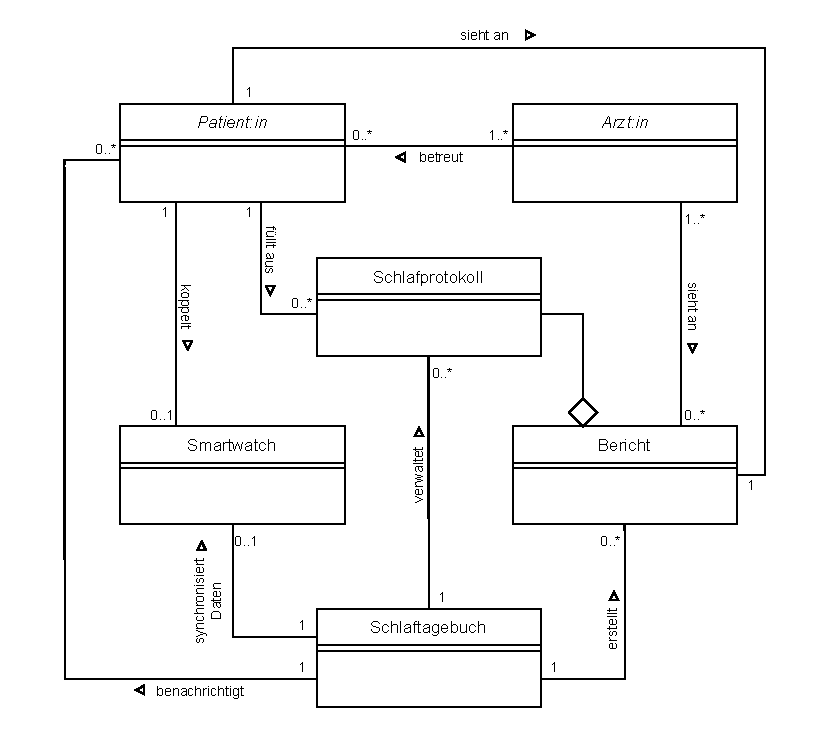
\includegraphics[width=0.8\textwidth]{images/meilenstein1/Klass.pdf} 
	\caption{Domänenstruktur: Schlaftagebuch}
	\label{fig:domänenstruktur}
\end{figure}

Eine Patient:in füllt regelmäßig Schlafprotokolle aus; jedes Protokoll gehört genau einer 
Patient:in (0..*\,→\,1), während eine Patient:in beliebig viele Protokolle besitzen kann (Im besten Fall aber nur 14).
Diese Protokolle werden im Schlaftagebuch gesammelt. \\

Optional kann eine Smartwatch mit einer Patient:in gekoppelt werden (Patient:in 1\,→\,0..1
Smartwatch). Sie stellt automatisch erfasste Schlafdaten bereit, die mit dem Schlaftagebuch
synchronisiert werden können. \\

Aus einem oder mehreren Schlafprotokollen wird ein Bericht erstellt. Die Aggregationsbeziehung
zeigt, dass ein Bericht Protokolle zusammenfasst, die jedoch unabhängig weiterexistieren
können. Eine Ärzt:in erhält diese Berichte zur Auswertung und betreut die jeweilige Patient:in
(Ärzt:in 1\,→\,0..* Patient:innen).

\newpage

\subsection{Geschäftsprozess}
Der Geschäftsprozess beschreibt den Ablauf der Schlafdiagnostik für Jugendliche im Schlaflabor. Ziel ist es, Schlafstörungen zu erkennen und eine Diagnose zu stellen. Die Software unterstützt diesen Prozess, 
indem sie digitale Schlafprotokolle sammelt, vervollständigt, validiert und in einem automatisch generierten Bericht zusammenfasst. Ärzt:innen nutzen diesen Bericht zur Auswertung und zur Erstellung einer Diagnose.

\begin{figure}[h]
	\centering
	\includegraphics[width=0.6\textwidth]{images/meilenstein1/Aktivität.pdf} 
	\caption{Geschäftsprozessdiagramm: Schlaftagebuch}
	\label{fig:activitydiagramgeneral}
\end{figure}

\newpage 

\subsection{Systemfunktionen}

\subsubsection{Übersicht}
Die dargestellte Use-Case-Diagramm zeigt die zentralen Systemfunktionen des Schlaftagebuchs aus der Perspektive der beiden Hauptakteure: \textbf{Patient:in} und \textbf{Arzt:in}. 
Es veranschaulicht, welche Aktionen die jeweiligen Nutzergruppen mit dem System durchführen können und wie sie mit den Kernfunktionalitäten interagieren.\\
Patient:innen sind die primären Anwender:innen des Systems. Sie können sich im Schlaftagebuch anmelden, ihre Einstellungen verwalten und eine Smartwatch mit dem System koppeln, 
um Schlafdaten automatisiert zu erfassen. Darüber hinaus haben Patient:innen die Möglichkeit, täglich ein Schlafprotokoll auszufüllen, in dem subjektive und objektive Angaben zum Schlafverhalten erfasst werden. \\
Ärzt:innen nutzen das System vor allem zur Einsicht und Auswertung der protokollierten Daten. 
Sie können die von Patient:innen erstellten PDF-Berichte ansehen, um einen Überblick über Schlafmuster, Auffälligkeiten und relevante Gesundheitsinformationen zu erhalten. \\

\begin{figure}[h]
	\centering
	\includegraphics[width=0.7\textwidth]{images/meilenstein1/usecase.pdf} 
	\caption{Use-Case-Diagramm: Schlaftagebuch}
	\label{fig:usecasediagram}
\end{figure}

\newpage

\subsubsection{Beschreibung pro Use Case}

\subsubsection*{Use Case: Anmelden}
\textbf{Titel:} Anmelden

\textbf{Kurzbeschreibung:}  
Aktivierung und Anmeldung des Nutzerkontos mithilfe eines einmaligen Zugangscodes.

\textbf{Aktoren:}  
Nutzer:in (Patient:in oder Ärzt:in)

\textbf{Vorbedingungen:}  
Ein einmaliger Zugangscode liegt vor.

\textbf{Ablauf:}  

1. Patient:in gibt den Zugangscode ein.  

2. System aktiviert das Nutzerkonto.  

3. Patient:in meldet sich an.

\textbf{Auswirkungen:}  
Nutzerkonto wird freigeschaltet und ist vollständig nutzbar.

\textbf{Anmerkungen:}  
Bei falschem Zugangscode erscheint eine Fehlermeldung.



\subsubsection*{Use Case: Einstellungen verwalten}

\textbf{Titel:} Einstellungen verwalten

\textbf{Kurzbeschreibung:}  
Änderung der Sprache und der täglichen Benachrichtigungszeit.

\textbf{Aktoren:}  
Patient:in

\textbf{Vorbedingungen:}  
Nutzerkonto ist angemeldet.

\textbf{Ablauf:}  

1. Öffnen des Einstellungsbereichs.

2. Auswahl der gewünschten Sprache.

3. Festlegung der täglichen Erinnerungszeit.

4. System speichert die neuen Einstellungen.

\textbf{Auswirkungen:}  
App-Sprache und Benachrichtigungen passen sich an.

\textbf{Anmerkungen:}  
Einstellungen können jederzeit geändert werden.

\clearpage 

\subsubsection*{Use Case: Smartwatch koppeln}

\textbf{Titel:} Smartwatch koppeln

\textbf{Kurzbeschreibung:}  
Verbindung der App mit einer kompatiblen Smartwatch zur automatischen Synchronisation von Schlafdaten.

\textbf{Aktoren:}  
Patient:in

\textbf{Vorbedingungen:}  
Eine Smartwatch ist vorhanden und eingeschaltet.

\textbf{Ablauf:}  

1. Patient:in startet den Kopplungsvorgang.

2. App sucht verfügbare Geräte.

3. Patient:in wählt die Smartwatch aus.

4. System stellt die Verbindung her.

\textbf{Auswirkungen:}  
Nutzerkonto wird freigeschaltet und ist vollständig nutzbar.

\textbf{Anmerkungen:}  
Bei falschem Zugangscode erscheint eine Fehlermeldung.



\subsubsection*{Use Case: Schlafprotokoll ausfüllen}

\textbf{Titel:} Schlafprotokoll ausfüllen

\textbf{Kurzbeschreibung:}  
Tägliche Eingabe der subjektiven und objektiven Angaben zum Schlaf.

\textbf{Aktoren:}  
Patient:in

\textbf{Vorbedingungen:}  
Nutzerkonto ist angemeldet.

\textbf{Ablauf:}  

1. Öffnen des Formulars für den aktuellen Tag.

2. Eintragen von Schlafdauer, Einschlafzeit und Aufwachzeit.

3. Bewertung der Schlafqualität und des Wohlbefindens.

4. System speichert das Protokoll.

\textbf{Auswirkungen:}  
Das Tagesprotokoll ist vollständig gespeichert.

\textbf{Anmerkungen:}  
Pro Tag kann nur ein Protokoll abgegeben werden.

\clearpage 

\subsubsection*{Use Case: Bericht ansehen}

\textbf{Titel:} Bericht ansehen

\textbf{Kurzbeschreibung:}  
Ärzt:in öffnet den automatisch generierten Bericht über die Schlafdaten.

\textbf{Aktoren:}  
Ärzt:in

\textbf{Vorbedingungen:}  
Ein Bericht wurde erstellt und die Ärzt:in ist autorisiert.

\textbf{Ablauf:}  

1. Ärzt:in öffnet die Berichtsübersicht.

2. Auswahl eines gewünschten Berichts.

3. System lädt und zeigt das Dokument.

\textbf{Auswirkungen:}  
Ärzt:in kann Schlafmuster analysieren und diagnostische Einschätzungen treffen.

\textbf{Anmerkungen:}  
Zugriff nur auf Berichte der zu betreuenden Patient:innen.

\newpage

\subsection{Beschreibung Systemtests}
\begin{itemize}
    \item \textbf{Ein Systemtest pro Use Case} für den Standardablauf
    \item Zusätzliche Tests für \textbf{alternative Abläufe}
\end{itemize}

\begin{figure}[h]
	\centering
	\includegraphics[width=0.7\textwidth]{images/meilenstein1/systemtests.png} 
	\caption{Systemtests}
	\label{fig:systemtests}
\end{figure}

